\Titre{Organisation de la Sécurité Informatique en France}

\let\oldemph=\emph
\def\emph#1{\oldemph{\textcolor{red}{#1}}}
\usetikzlibrary{positioning}
  
\usepackage{ifthen}


\def\txthl#1{ \ifthenelse{\lengthtest{#1 pt<0.5pt}}{\top}{\bot} }

\usetikzlibrary{shapes,fit}

\def\codelegal#1{%
  \tikz{%
    \node[draw=red!60!black,rounded corners=.5ex,inner sep=3pt]   (text)  {#1\hspace*{1em}};%
    \node[yshift=-0.5ex] at (text.north east) {
\includegraphics[width=1em]{images/icone_code.jpg}} ;%
  }%
}

\tikzstyle{-|}=[to path={-| (\tikztotarget)}]
\tikzstyle{|-}=[to path={|- (\tikztotarget)}]
\tikzstyle{itembook}=[
  draw=red!60!black,
  rounded corners=.5ex,
  inner sep=3pt
]
\tikzstyle{organisme}=[
  draw=red!60!black,
  rounded corners=.5ex,
  inner sep=1ex,
  fill=blue!50!red!60!green!30,
  fill opacity=.05,
  text opacity=1,
  thick
]
\tikzstyle{organismewh}=[%
  draw=red!60!black,
  opacity=1,
  rounded corners=.5ex,
  inner sep=1ex,
  thick,
  rectangle split, 
%  rectangle split horizontal, 
  rectangle split parts=2,
  fill=blue!50!red!60!green!30,
  fill opacity=.05,
  text opacity=1
]

\def \organisme#1{%
  \tikz{%
    \node[organisme]  {#1};%
  }%
}
\def \organismewh#1#2{%
  \tikz{%
    \node[organismewh] {#1\nodepart{two} #2};%
  }%
}

\begin{document}

\begin{reveals}
		
\maketitle

\section{Organisation de la cybersécurité en France}

\begin{frame}
  \frametitle{Cyberdéfense}

  \vfill
  \begin{center}
    
\includegraphics[width=0.3\textwidth]{images/livre_blanc_defense.jpg}%
    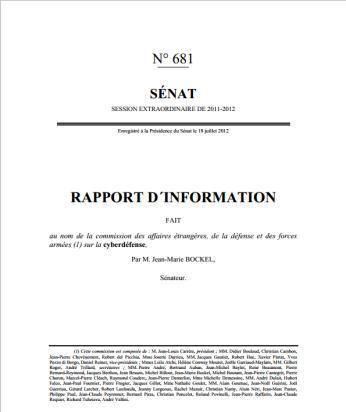
\includegraphics[width=0.3\textwidth]{images/rapport_information_senat.jpg}%
    
\includegraphics[width=0.3\textwidth]{images/projet_loi_programmation_militaire-2014-2019.jpg}%
  \end{center}

  \vfill
  \begin{block}{Principaux points}
    \begin{itemize}
    \item cyberattaques, une menace majeure
    \item besoin d'un effort marqué (libre blanc 2013)
    \end{itemize}
  \end{block}

  \vfill

\end{frame}

\begin{frame}
  \frametitle{Organisation de la sécurité en France}
  \footnotesize
  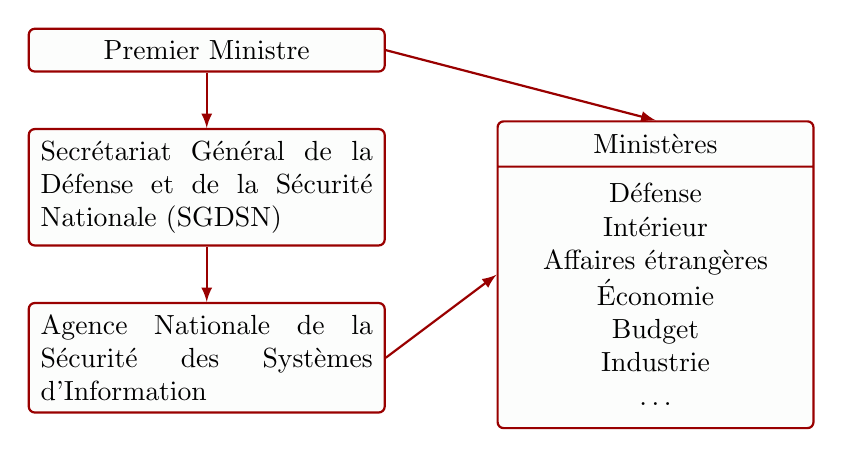
\begin{tikzpicture}[node distance=2em and 4em]
    \node[organismewh] (ministeres) {Ministères \nodepart{two} \begin{tabular}{c} \hspace*{3em}Défense\hspace*{3em}\\Intérieur\\Affaires étrangères\\Économie\\Budget\\Industrie\\\(\ldots\)\\\end{tabular}} ;
    \node[organisme,left=of ministeres.west,yshift=-3em] (anssi)  {\parbox{12em}{Agence Nationale de la Sécurité des Systèmes d'Information}} ;
    \node[organisme,above =of anssi.north] (sgdsn){\parbox{12em}{Secrétariat Général de la Défense et de la Sécurité Nationale (SGDSN)}} ;
    \node[organisme,above =of sgdsn.north] (pm){\parbox{12em}{\hfil Premier Ministre\hfil}} ;
    \draw[>=latex,->,draw=red!60!black,thick] (pm.east) -- (ministeres.north);
    \draw[>=latex,->,draw=red!60!black,thick] (pm.south) -- (sgdsn.north);
    \draw[>=latex,->,draw=red!60!black,thick] (sgdsn.south) -- (anssi.north);
    \draw[>=latex,->,draw=red!60!black,thick] (anssi.east) -- (ministeres.west);
  \end{tikzpicture}
  \begin{trivlist}
  \item \textbf{Hauts fonctionnaires de défense et de sécurité
      (HFDS):} préparation, coordination des mesures de défense,
    chargés de la sécurité des SI
  \end{trivlist}
\end{frame}



\setbeamercolor{background canvas}{bg=white}
\begin{frame}

  \hspace*{-.5em}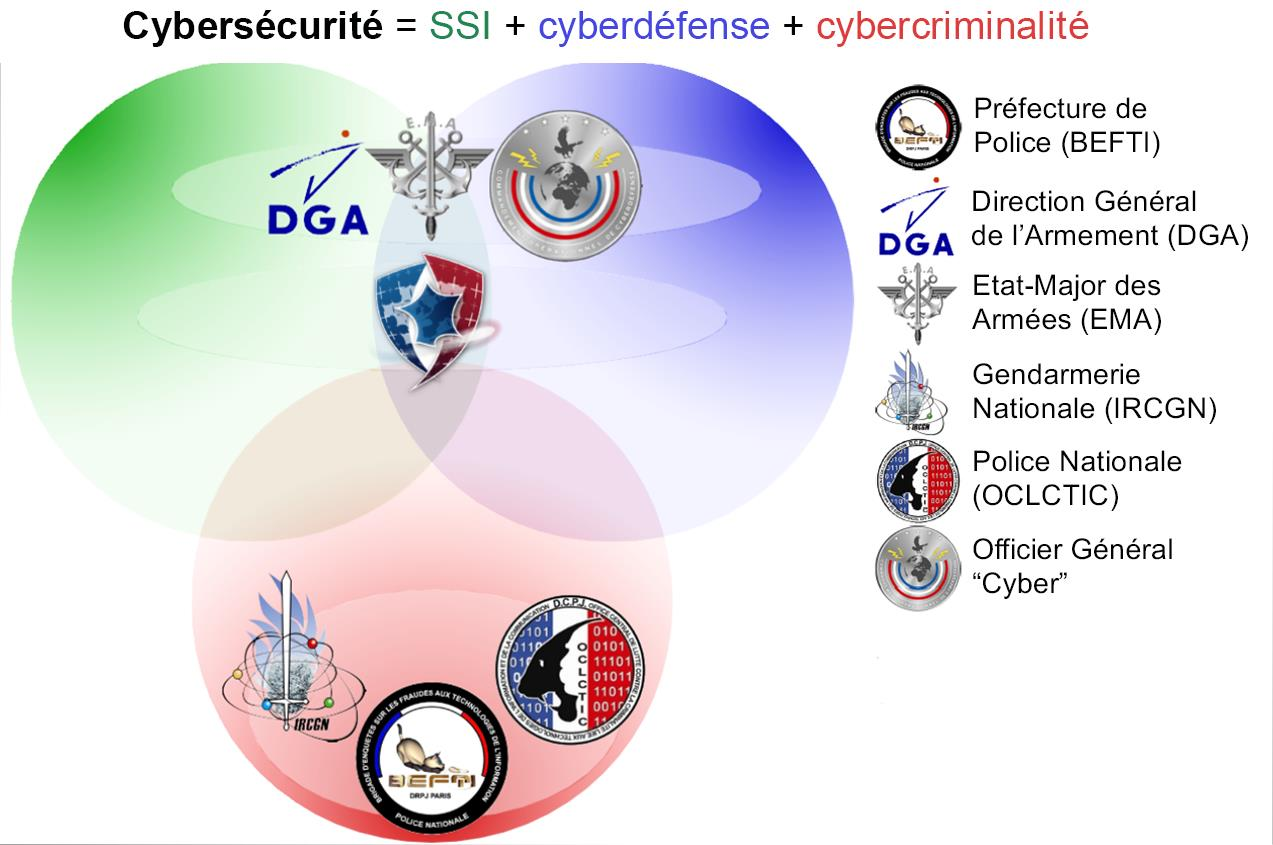
\includegraphics[width=1\textwidth]{images/cybersecurite.jpg}

  \frametitle{Cybersécurité}


\end{frame}

\section{Législation}

\begin{frame}
  \frametitle{Domaines couverts}

  \begin{itemize}
  \item Liberté d'expression
  \item Protection du \textit{e}-commerce
  \item Propriété intellectuelle
  \item Protection de la vie privée
  \item protection des entreprises
  \item Cybercriminalité
  \item \(\ldots\)
  \end{itemize}
\end{frame}

\begin{frame}
  \frametitle{Textes légaux}

  \begin{columns}
    \begin{column}{0.6\textwidth}
      \begin{itemize}
      \item Un droit \emph{non codifié}: des dizaines de codes en vigueur
      \item \(\ldots\) et difficile d'accès
        \begin{itemize}
        \item au carrefour des autres droits
        \item en évolution constante et rapide
        \item issu de textes de toute nature/niveaux
        \item beaucoup de jurisprudence
        \end{itemize}
      \item besoin d'un effort de veille juridique 
      \end{itemize}      
    \end{column}
    \begin{column}{0.27\textwidth}
      \codelegal{\parbox{\textwidth}{Code de la défense}}
      \codelegal{\parbox{\textwidth}{Code civil}}
      \codelegal{\parbox{\textwidth}{Code pénal}}
      \codelegal{\parbox{\textwidth}{Droit du travail}}
      \codelegal{\parbox{\textwidth}{Code de la propriété intellectuelle}}
      \codelegal{\parbox{\textwidth}{Code des postes\& comm. élect.}}
      \codelegal{\parbox{\textwidth}{Code de la consommation}}
      \codelegal{\parbox{\textwidth}{\(\ldots\)}}
    \end{column}
  \end{columns}

\end{frame}

\section{Cybercriminalité}

\begin{frame}
  \frametitle{Lutte contre la cybercriminalité}

  \vfill
  \begin{block}{Définition}
    Ensemble des actes contrevenants aux traités internationaux ou aux
    lois nationales utilisant les réseaux ou les systèmes
    d'information comme moyens de réalisation d’un délit ou d'un
    crime, ou les ayant pour cible.
  \end{block}
  \vfill
  \begin{block}{Investigation numérique (\emph{forensics})}
    Ensemble des protocoles et de mesures permettant de rechercher des
    éléments techniques sur un conteneur de données numériques en vue
    de répondre à un objectif technique en respectant une procédure de
    préservation du conteneur.
  \end{block}
\end{frame}

\begin{frame}
  \frametitle{État de la législation (1/2)}
  \vfill
  \begin{block}{Loi Godfrain du 05/01/1988}
    \small L'\emph{accès} ou le \emph{maintien} frauduleux dans tout ou partie d'un système de traitement automatisé des données (STAD), art. 323-1 du code pénal, est puni de 2 ans d'emprisonnement et de 30.000\euro\ d'amende au maximum.
  \end{block}
  \vfill
  \begin{block}{Commentaires}
    \small
    \begin{itemize}
    \item élément matériel de l'infraction: accès ou maintien
    \item fraude ou l'élément moral: être connaissance d'être sans droit et en connaissance de cause
    \end{itemize}
  \end{block}
  \vfill
  \begin{block}{Jurisprudence}\small
    \begin{itemize}
    \item définition des STAD: réseau d'un fournisseur, réseau bancaire, disque dur, radio, téléphone, site internet,\ldots
    \item tendance des tribunaux: plus grande intransigeance envers
      les hébergeurs ne protégeant pas assez les données de leurs
      utilisateurs
    \end{itemize}
  \end{block}
  \vfill
\end{frame}

\begin{frame}
  \frametitle{État de la législation (2/2)}
  \vfill
  \begin{block}{Article 323-2 du code pénal}\small 
    \emph{Entraver ou fausser} le fonctionnement d'un STAD est puni
    d'un maximum de 5 ans d'emprisonnement et de 75.000\euro\ d'amende
  \end{block}
  \vfill
  \begin{block}{Article 323-3 du code pénal}\small 
    \emph{L'introduction, la suppression ou la modification
      frauduleuse de données} dans un STAD est puni d'un maximum de 5
    ans d'emprisonnement et de 75.000\euro\ d'amende
  \end{block}
  \vfill
  \begin{block}{Article 323-3-1 du code pénal}\small 
    \emph{Importer, détenir, offrir, céder, mettre à disposition} sans
    motif légitime un programme ou un moyen permettant de commettre
    une\! de\! ces\! infractions\! est\! puni\! de\! la même peine
  \end{block}
  \vfill
  \scriptsize
  \begin{itemize}
  \item Art. 323-4: association de malfaiteurs en informatique
  \item Art. 323-5: peines complémentaires
  \item Art. 323-6: responsabilité pénale des personnes morales
  \item Art. 323-7: répression de la tentative
  \end{itemize}
  \vfill
\end{frame}
\section{Protection des données personnelles}

\begin{frame}
  \frametitle{Rôle de la CNIL}

  \vfill
  \begin{block}{Origine}
    Loi du 06/01/1978 relative à l'informatique, aux fichiers, et aux libertés
  \end{block}
  \vfill
  \begin{block}{Champ d'application (Art. 2)}
    \small La présente loi s'applique aux \emph{traitements
      automatisés} de données à caractère personnel, ainsi qu’aux
    \emph{traitements non automatisés} de données à caractère
    personnel contenues ou appelées à figurer dans des fichiers, à
    l'exception des traitements mis en \oe uvre pour l’exercice
    d’activités exclusivement personnelles, lorsque leur
    \emph{responsable} remplit les conditions prévues à l’article 5
    (relevant du droit national).
  \end{block}
  \vfill
  \begin{block}{Qu'est-ce qu'une donnée à caractère personnel ?}\small
    Constitue une donnée à caractère personnel toute
    \emph{information} relative à une \emph{personne physique}
    identifiée \emph{ou qui peut être identifiée}, \emph{directement
      ou indirectement}, par référence à un numéro d’identification ou
    à un ou plusieurs éléments qui lui sont propres.
  \end{block}
  \vfill
\end{frame}

\begin{frame}
  \frametitle{Protection des données à caractère personnel}
  \vfill
  \begin{block}{Traitement \emph{loyal et licite}}\small
    \begin{itemize}
    \item les données sont collectées pour des \emph{finalités
        déterminées} explicites et légitimes
    \item de manière \emph{proportionnée} (adéquates, pertinentes, et
      non excessives)
    \item avec le \emph{consentement de la personne concernée} (sauf
      exception)
    \item pendant une durée \emph{n'excédant pas celle nécessaire à la
        réalisation des finalités}
    \end{itemize}
  \end{block}
  \vfill
  \begin{block}{Droits des personnes physiques sur leurs données}\small
    \begin{itemize}
    \item Un droit d'\emph{information} préalable au consentement 
    \item Un droit d'\emph{accès} aux données collectées
    \item Un droit de \emph{rectification}
    \item Un droit d\emph{opposition} pour raison légitime
    \end{itemize}
  \end{block}
\end{frame}

\begin{frame}
  \frametitle{Obligations administratives}
  \vfill
  \begin{block}{Déclaration préalable (Art. 22 à 24)}\small
    \begin{itemize}
    \item Le traitement peut faire l'objet d'une dispense de déclaration
    \item Le traitement échappe à l'obligation de déclaration car le
      responsable du traitement a désigné un correspondant à la
      protection des données (CIL)
    \item Dans tous les autres cas, le traitement doit effectivement
      faire l'objet d'une déclaration préalable
    \end{itemize}
  \end{block}
  \vfill
  \begin{block}{Autorisation préalable (Art. 25 à 27)}\small
    \begin{itemize}
    \item pour les traitements sensibles listés à l'article 25
    \item examen par la CNIL sous deux mois (\emph{whitelisting},
      rejet si pas de réponse positive)
    \end{itemize}
  \end{block}
  \vfill
\end{frame}

\begin{frame}
  \frametitle{Obligations de confidentialité et de sécurité}
  \vfill
  \begin{block}{Pour l'opérateur principal}\small
    \begin{itemize}
    \item mise en \oe uvre des mesures techniques et
      organisationnelles appropriées, au regard de la nature des
      données et des risques, pour préserver leur sécurité
    \item sécurité: empêcher qu'elles soient déformées, endommagées,
      ou que des tiers non-autorisés y aient accès
    \item pas de techniques précisés dans le texte, mais un guide de
      sécurité est publié par la CNIL
    \end{itemize}
  \end{block}
  \vfill
  \begin{block}{Pour les sous-traitants}\small
    \begin{itemize}
    \item ils doivent apporter les mêmes garanties que l'opérateur principal
    \item sous la responsabilité de l'opérateur principal
    \end{itemize}
  \end{block}
  \vfill
\end{frame}

\begin{frame}
  \frametitle{Peines prévues}
   \vfill
   \begin{block}{Sanctions pénales}\small
    \begin{itemize}
    \item Douze délits punis de 3 à 5 ans d'emprisonnement et jusqu'à
      300.000\euro\ d'amende
    \item obligations de sécurité « Le fait de procéder ou de faire
      procéder à un traitement de données à caractère personnel sans
      mettre en \oe uvre les mesures prescrites à l'article 34 de la loi
      78-17 du 6 janvier 1978 précitée est puni de cinq ans
      d'emprisonnement et de 300 000\euro\ d'amende »
    \end{itemize}
  \end{block}
  \vfill
  \begin{block}{Sanctions civiles}\scriptsize
    Dommages-intérêts en fonction du préjudice causé aux personnes
    concernées
  \end{block}
  \vfill
  \begin{block}{Sanctions administratives par la CNIL}\scriptsize
    \begin{itemize}
    \item injonction de cesser le traitement pour les fichiers soumis
      à déclaration ou de retrait de l’autorisation accordée
    \item sanction pécuniaire
    \item interruption de la mise en \oe uvre du traitement ou
      verrouillage des données pour 3 mois
    \item publicité des avertissements et, en cas de mauvaise foi,
      pour les autres sanctions
    \end{itemize}
  \end{block}
  \vfill
\end{frame}


\end{reveals}
\end{document}
 
